\documentclass[8pt]{beamer}
\usepackage[cache=false]{minted}
\usepackage[utf8x]{inputenc}
\usepackage{hyperref}
\usepackage{fontawesome}
\usepackage{graphicx}
\usepackage[english,ngerman]{babel}
\usepackage{bussproofs}
\usepackage{dsfont}
\usepackage[all]{xy}

% ------------------------------------------------------------------------------
% Use the beautiful metropolis beamer template
% ------------------------------------------------------------------------------
\usepackage[T1]{fontenc}
\usepackage{fontawesome}
\usepackage{FiraSans}
\newtheorem{defin}{Definition}
\newtheorem{theor}{Theorem}
\newtheorem{prop}{Proposition}
\mode<presentation>
{
  \usetheme[progressbar=foot,numbering=fraction,background=light]{metropolis}
  \usecolortheme{default} % or try albatross, beaver, crane, ...
  \usefonttheme{default}  % or try serif, structurebold, ...
  \setbeamertemplate{navigation symbols}{}
  \setbeamertemplate{caption}[numbered]
  %\setbeamertemplate{frame footer}{My custom footer}
}

% ------------------------------------------------------------------------------
% beamer doesn't have texttt defined, but I usually want it anyway
% ------------------------------------------------------------------------------
\let\textttorig\texttt
\renewcommand<>{\texttt}[1]{%
  \only#2{\textttorig{#1}}%
}

% ------------------------------------------------------------------------------
% minted
% ------------------------------------------------------------------------------


% ------------------------------------------------------------------------------
% tcolorbox / tcblisting
% ------------------------------------------------------------------------------
\usepackage{xcolor}
\definecolor{codecolor}{HTML}{FFC300}

\usepackage{tcolorbox}
\tcbuselibrary{most,listingsutf8,minted}

\tcbset{tcbox width=auto,left=1mm,top=1mm,bottom=1mm,
right=1mm,boxsep=1mm,middle=1pt}

\newtcblisting{myr}[1]{colback=codecolor!5,colframe=codecolor!80!black,listing only,
minted options={numbers=left, style=tcblatex,fontsize=\tiny,breaklines,autogobble,linenos,numbersep=3mm},
left=5mm,enhanced,
title=#1, fonttitle=\bfseries,
listing engine=minted,minted language=r}


% ------------------------------------------------------------------------------
% Listings
% ------------------------------------------------------------------------------
\definecolor{mygreen}{HTML}{37980D}
\definecolor{myblue}{HTML}{0D089F}
\definecolor{myred}{HTML}{98290D}

\usepackage{listings}

% the following is optional to configure custom highlighting
\lstdefinelanguage{XML}
{
  morestring=[b]",
  morecomment=[s]{<!--}{-->},
  morestring=[s]{>}{<},
  morekeywords={ref,xmlns,version,type,canonicalRef,metr,real,target}% list your attributes here
}

\lstdefinestyle{myxml}{
language=XML,
showspaces=false,
showtabs=false,
basicstyle=\ttfamily,
columns=fullflexible,
breaklines=true,
showstringspaces=false,
breakatwhitespace=true,
escapeinside={(*@}{@*)},
basicstyle=\color{mygreen}\ttfamily,%\footnotesize,
stringstyle=\color{myred},
commentstyle=\color{myblue}\upshape,
keywordstyle=\color{myblue}\bfseries,
}

\setbeamercolor{emph}{fg=blue}
\renewcommand<>{\emph}[1]{%
  {\usebeamercolor[fg]{emph}\only#2{\itshape}#1}%
}

% ------------------------------------------------------------------------------
% The Document
% ------------------------------------------------------------------------------
\title{Intuitionistic epistemic logic categorically and algebraically}
\author{Daniel Rogozin \\ University College London}
\date{Seminar on Programming principles, Logic and Verification \\ The 24th of March 2023}
\begin{document}

\maketitle

\section{Introduction}

\begin{frame}
\frametitle{Intuitionistic modal logic: the big picture}
\begin{itemize}
\item As it is well known, modal logic extends classical logic with modal operators.
\item Applications: topology, proof theory, formal verification, ontologies, etc.
\item Intuitionistic modal logic is a version of modal logic where the underlying logic is the intuitionistic one.
\item Possible topics where intuitionistic modal logic is of interest:
\begin{itemize}
\item Constructive necessity, provability in intuitionistic arithmetic, intuitionistic knowledge, etc.
\item Model theory: the finite model property, canonicity \`a la Salqvist, definability \`a la Thomason-Goldblatt, etc.
\item Representation theory: general descriptive frames, Esakia duality, etc.
\end{itemize}
\end{itemize}
\onslide<2->{
See this summary paper to have the big picture in more detail
\begin{small}
\begin{itemize}
\item Frank Wolter and Michael Zakharyaschev. Intuitionistic Modal Logic, 1999.
\end{itemize}
\end{small}
}
\end{frame}


\begin{frame}
\frametitle{Modalities type theoretically}

\begin{itemize}
\item Type theory deals with a computation every value in which is annotated with the corresponding data type. Type theory is closely connected with intuitionistic logic and constructive proofs through the Curry-Howard correspondence.
\item One can extend Curry-Howard to intuitionistic modal logic and study modal operators within the ``types-as-formulas'' and ``proofs-as-terms'' paradigm.
\item Here we think of modal types as abstract data types of action, which are of interest for functional programming.
\end{itemize}

\onslide<2->{
\begin{small}
See the following:
\begin{itemize}
\item Gianluigi Bellin, Valeria De Paiva and Eike Ritter. Extended Curry-Howard Correspondence for a Basic Constructive Modal Logic, 2003
\item Frank Pfenning and Rowan Davies. A Judgmental Reconstruction of Modal Logic, 2000.
\item Peter Nicholas Benton, Gavin M. Bierman, Valeria de Paiva. Computational types from a logical perspective, 1998.
\item David Corfield. Modal homotopy type theory: The prospect of a new logic for philosophy, 2020.
\end{itemize}
\end{small}
}

\end{frame}

\section{Modal type theory based on ${\bf IEL}^-$}

\begin{frame}
\frametitle{Bridges with functional programming}
\end{frame}

\begin{frame}
\frametitle{The definition of the type theory}

The modal lambda calculus $\lambda_{{\bf IEL}^{-}}$ is axiomatised with the following inference rules.

\begin{center}
  \begin{prooftree}
  \AxiomC{$ $}
  \RightLabel{\scriptsize{ax}}
  \UnaryInfC{$\Gamma, x : \varphi \vdash x : \varphi$}
  \end{prooftree}
  \end{center}

  \begin{minipage}{0.45\textwidth}
    \begin{prooftree}
    \AxiomC{$\Gamma, x : \varphi \vdash M : \psi$}
    \RightLabel{$\rightarrow_i$}
    \UnaryInfC{$\Gamma \vdash \lambda x. M : \varphi \to \psi$}
    \end{prooftree}

    \begin{prooftree}
    \AxiomC{ $\Gamma \vdash M : \varphi$ }
    \AxiomC{ $\Gamma \vdash N : \psi$ }
    \RightLabel{$\times_i$}
    \BinaryInfC{$\Gamma \vdash \langle M, N \rangle : \varphi \times \psi$}
    \end{prooftree}

    \begin{prooftree}
      \AxiomC{$\Gamma \vdash M : \varphi$}
      \RightLabel{$\bigcirc_I$}
      \UnaryInfC{$\Gamma \vdash {\bf pure \: } \: M : \bigcirc \varphi$}
    \end{prooftree}
\end{minipage}%
\hfill
\begin{minipage}{0.45\textwidth}
\begin{tabular}{p{\textwidth}}
  \begin{prooftree}
  \AxiomC{$\Gamma \vdash M : \varphi \to \psi$}
  \AxiomC{$\Gamma \vdash N : \varphi$}
  \RightLabel{$\rightarrow_e$}
  \BinaryInfC{$\Gamma \vdash M N : \psi$}
  \end{prooftree}

  \begin{prooftree}
  \AxiomC{ $\Gamma \vdash M : \varphi_1 \times \varphi_2$ }
  \RightLabel{$\times_e$, $i = 1, 2$}
  \UnaryInfC{$\Gamma \vdash \pi_i M : \varphi_i$}
  \end{prooftree}

  \begin{prooftree}
    \AxiomC{$\Gamma \vdash \overrightarrow{M} : \bigcirc \overrightarrow{\varphi}$}
    \AxiomC{$\overrightarrow{x} : \overrightarrow{\varphi} \vdash N : \psi$}
    \RightLabel{$\text{let}_{\bigcirc}$}
    \BinaryInfC{$\Gamma \vdash {\bf let \:} \bigcirc \overrightarrow{x} = \overrightarrow{M} {\: \bf in \: } N : \bigcirc \psi$}
  \end{prooftree}
\end{tabular}
\end{minipage}%

\end{frame}

\begin{frame}
\frametitle{Reduction rules}

The reduction rules are defined with the following rewriting rules:

\begin{enumerate}
  \item $(\lambda x. M) N \rightarrow_{\beta} M [x := N]$.
  \item $\pi_1 \langle M, N \rangle \rightarrow_{\beta} M$.
  \item $\pi_2 \langle M, N \rangle \rightarrow_{\beta} N$.
  \item ${\bf let \:} \bigcirc \vec{x}, y, \vec{z} = \vec{M}, {\bf let \:} \bigcirc \vec{w} = \vec{N} {\: \bf in \: } Q, \vec{P} {\: in \:} R \rightarrow_{\beta}
  {\bf let \:} \bigcirc \vec{x}, \vec{w}, \vec{z} = \vec{M}, \vec{N}, \vec{P} {\: \bf in \: } R [y := Q]$.
  \item ${\bf let \:} \bigcirc \vec{x} = {\bf pure \:} \vec{M} {\: \bf in \:} N \rightarrow_{\beta} {\bf pure \:} N [\vec{x} := \vec{M}]$.
  \item ${\bf let \:} \bigcirc \underline{\quad} = \underline{\quad} {\: \bf in \:} M \rightarrow_{\beta} {\bf pure \:} M$, where \underline{\quad} is an empty sequence of terms.
\end{enumerate}

\onslide<2->{
The multistep reduction $\twoheadrightarrow_{\beta}$ is reflexive-transitive closure of $\rightarrow_{\beta}$.
}

\end{frame}

\begin{frame}
\frametitle{Metatheoretic properties}

\begin{theorem} [D.R. 2018]

\begin{enumerate}
\item (Type preservation)

If $\Gamma \vdash M : \varphi$ and $M \twoheadrightarrow_{\beta} N$, then $\Gamma \vdash N : \varphi$
\item (Strong normalisation)

Every reduction path terminates, that is, no infinite reduction sequences.
\item (Church-Rosser)

If $M \twoheadrightarrow_{\beta} N_1, N_2$, then there exists $P$ such that $N_1, N_2  \twoheadrightarrow_{\beta} P$.
\end{enumerate}
\end{theorem}

As a corollary, every $\lambda_{{\bf IEL}^- term}$ has a unique normal form.
\end{frame}

\section{Categorical completeness}

\begin{frame}
\frametitle{Category theory}

Now I am going to be like the guy from the right.
\begin{center}
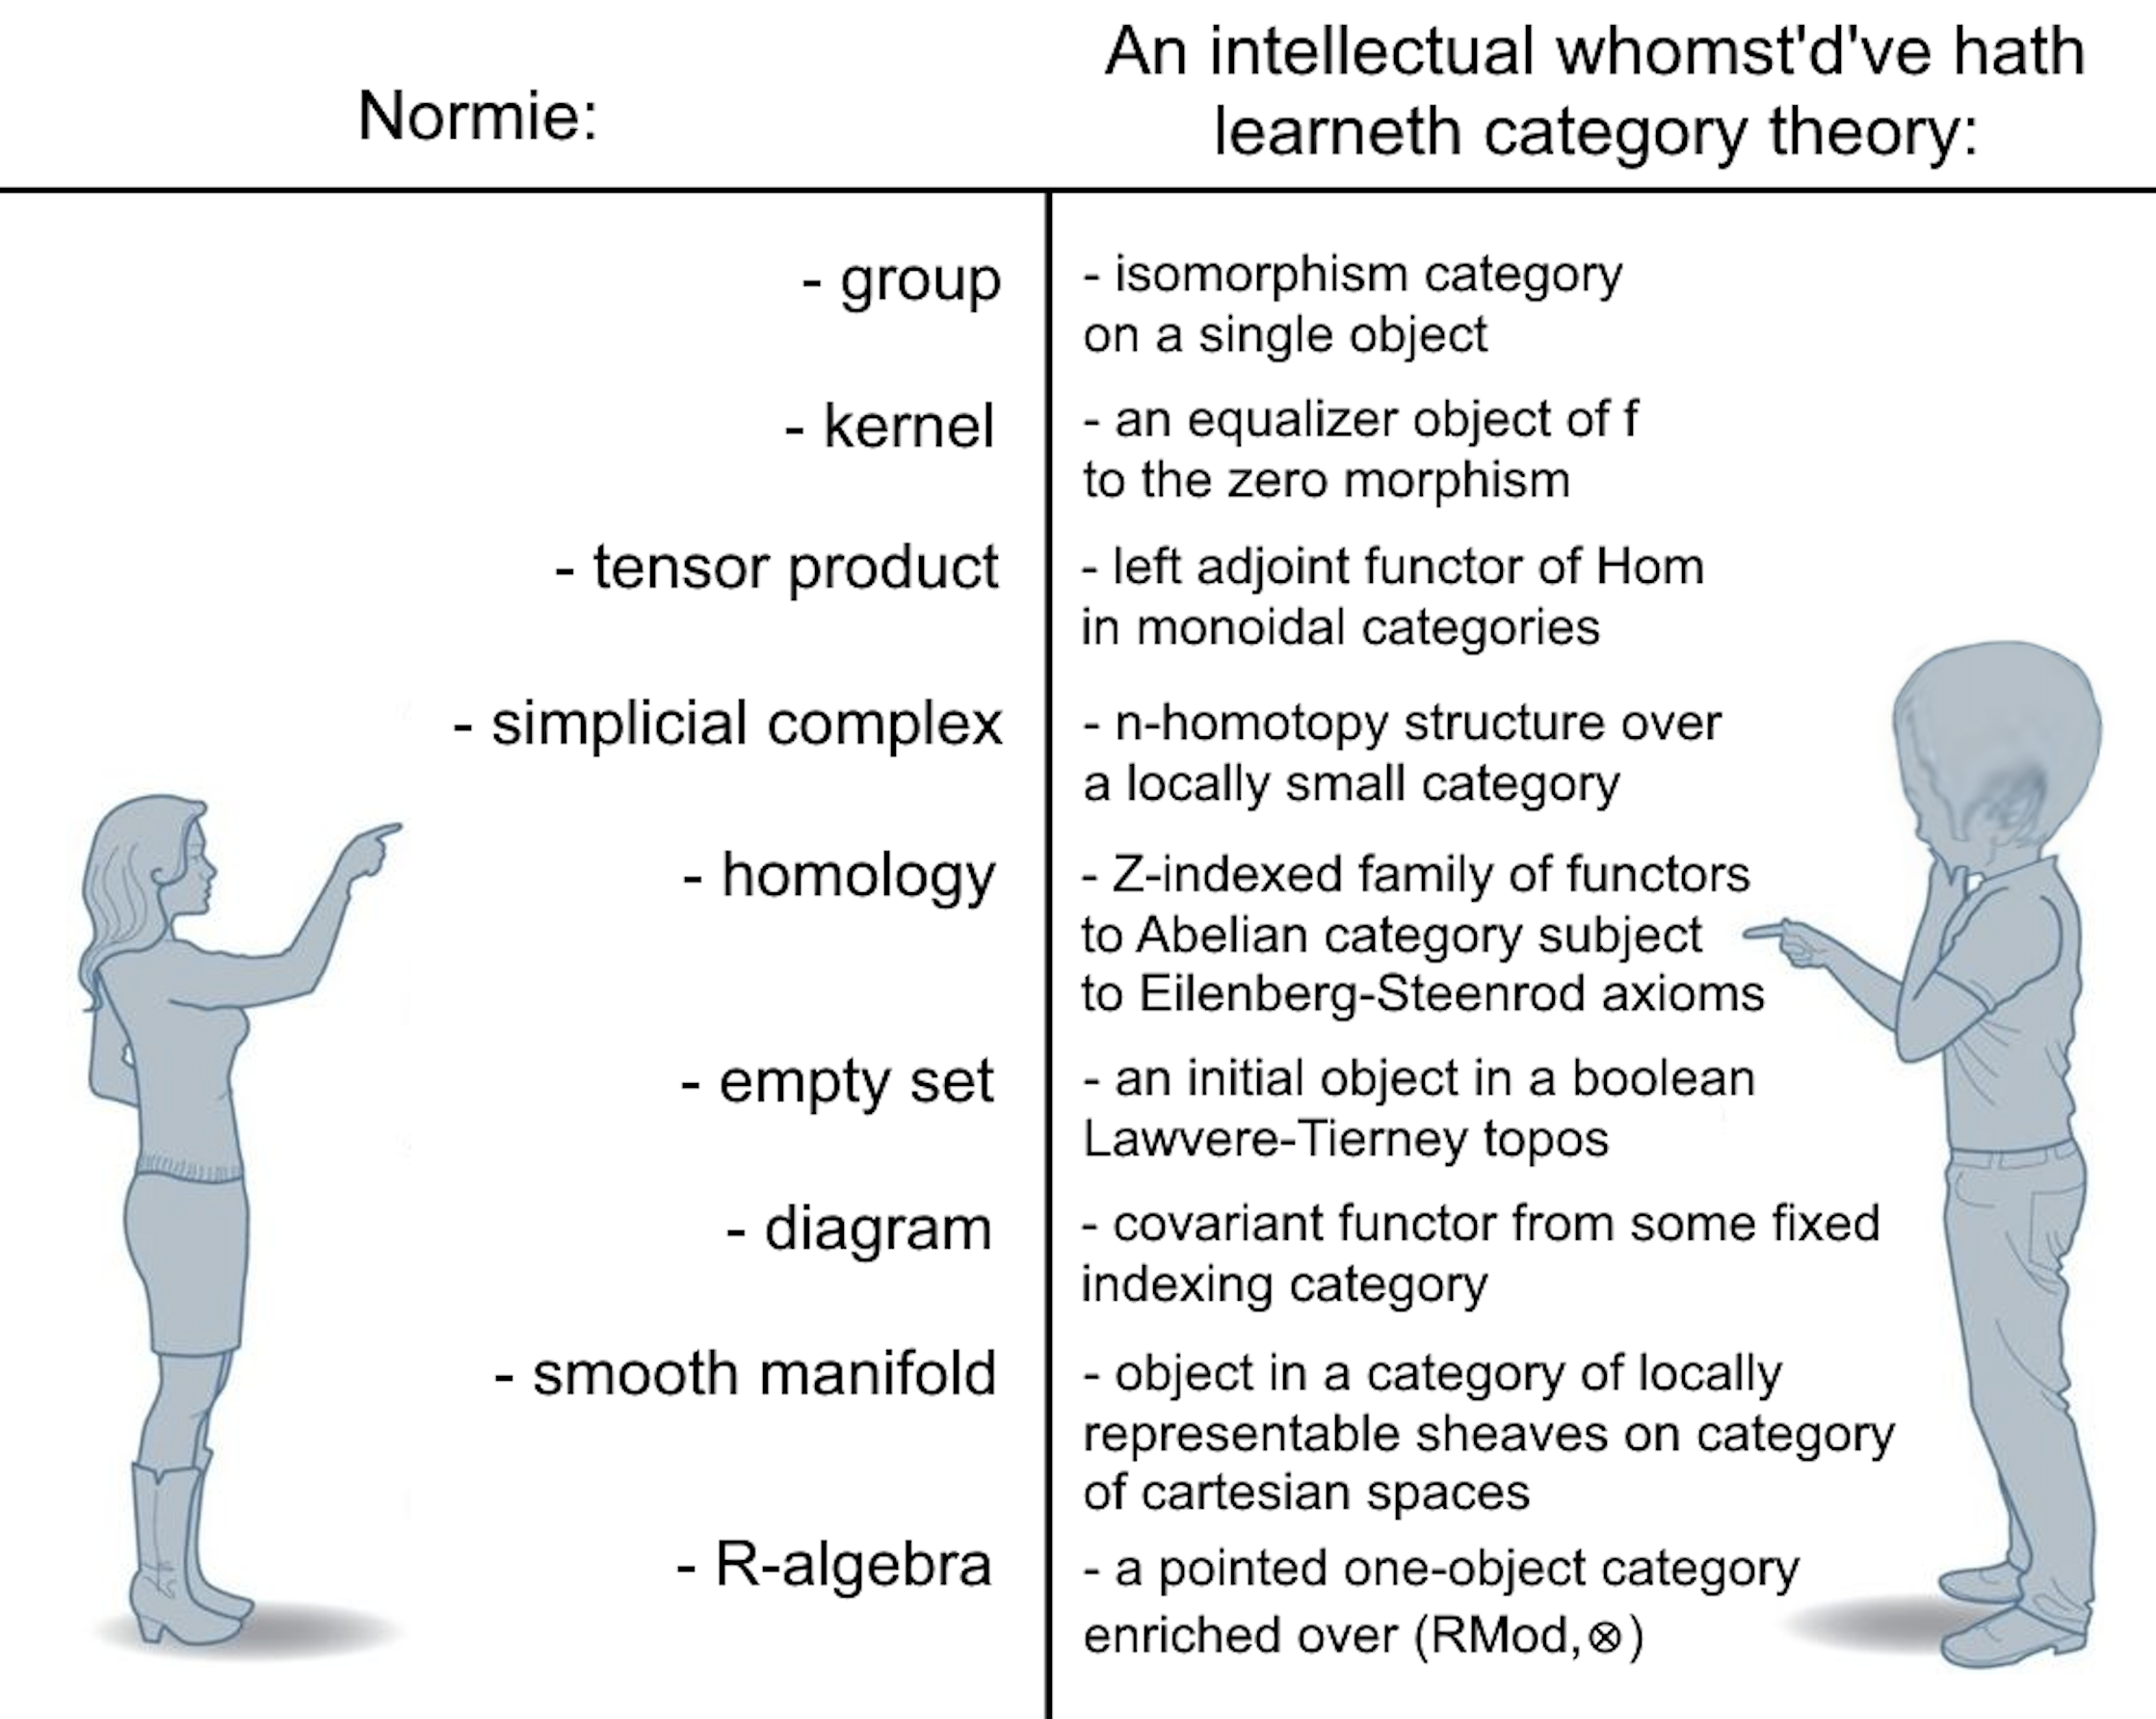
\includegraphics[scale=0.225]{meme.png}
\end{center}

\end{frame}

\begin{frame}
\frametitle{General concepts: Category}
Recall that a category $\mathcal{C}$ consists of:
\begin{itemize}
\item A class of objects $\operatorname{Ob}(\mathcal{C}) = \{ A, B, C, \dots \}$,
\item A class of morphisms $\mathcal{C}(A, B)$ for each $A, B \in \operatorname{Ob}(\mathcal{C})$, where $f : A \to B$ iff $f \in \mathcal{C}(A, B)$,
\item For $f : A \to B$ and $g : B \to C$, then $g \circ f : A \to C$ and $h \circ (g \circ f) = (h \circ g) \circ f$ for each $f, g, h$ having an appropriate domain and codomain,
\item For each $A, B \in \operatorname{Ob}(\mathcal{C})$ we have identity morphisms such that for each $f : A \to B$ $f \circ id_A = f$ and $id_B \circ f = f$.
\end{itemize}
\onslide<2->{
Some examples:
\begin{itemize}
\item ${\bf Set}$, the category of all sets and all functions betweem them,
\item ${\bf Top}$, the category of all topological spaces and continuous maps,
\item ${\bf Vect}_k$, the category of vector spaces over a field $k$ and linear maps,
\item $(P, \leq)$, any poset where $a \to b$ exists iff $a \leq b$,
\item Any monoid (as well as a group) is a category, where $\operatorname{Ob}(\mathcal{C})$ is a singleton set (Cayley's theorem).
\item etc.
\end{itemize}}
\end{frame}

\begin{frame}
\frametitle{General concepts: Functor}

Intuitively, a functor is a morphism of category. Rigorously, let $\mathcal{C}$ and $\mathcal{D}$ be categories, a functor ${\bf F} : \mathcal{C} \to \mathcal{D}$ is a ``function'' such that:
\begin{itemize}
\item Each $A \in \operatorname{Ob}(\mathcal{C})$ maps to ${\bf F} A \in \operatorname{Ob}(\mathcal{D})$,
\item Each $f : A \to B$ in $\mathcal{C}$ maps to ${\bf F} f : {\bf F} A \to {\bf F} B$ in $\mathcal{D}$,
\item ${\bf F} (id_A) = id_{{\bf F} A}$
\item ${\bf F}  (g \circ f) = {\bf F} g \circ {\bf F} f$ for each $f$ and $g$.
\end{itemize}
\onslide<2->{
Some examples:
\begin{itemize}
\item The powerset functor $\mathcal{P} : {\bf Set} \to {\bf Set}$ such that $\mathcal{P} : A \mapsto 2^{A}$,
\item The abelianisation functor $Ab : {\bf Group} \to {\bf Ab}$ such that $Ab : G \mapsto G / [G, G]$,
\item The spectrum functor $\operatorname{Spec} : {\bf Ring}^{op} \to {\bf Top}$ that maps every commutative ring to its Zariski space,
\item ${\bf Field} \to {\bf Ring}$ such that $k \mapsto k[X]$,
\item $\pi_1 : {\bf Top}_* \to {\bf Group}$ maps every topological space with a base point to its fundamental group, for example, $\pi_1(S) = \mathbb{Z}$ (up to isomorphism).
\item etc.
\end{itemize}}
\end{frame}

\begin{frame}
\frametitle{General concepts: Natural transformation}
A natural transformation is a functor morphism. Let $\mathcal{C}, \mathcal{D}$ be categories and ${\bf F}, {\bf G} : \mathcal{C} \to \mathcal{D}$ functors. A natural tranformation $\theta : {\bf F} \Rightarrow {\bf G}$ is a collection of morphisms $\theta_A : {\bf F} A \to {\bf G} A$ in $\mathcal{D}$ making the following square commute for each $f : A \to B$ and $A, B \in \operatorname{Ob}(\mathcal{C})$:
\centerline{
\xymatrix{
{\bf F} A \ar[rr]^{{\bf F} f} \ar[d]_{\theta_A} && {\bf F} B \ar[d]^{\theta_B} \\
{\bf G} A \ar[rr]_{{\bf G} f} && {\bf G} B
}}

\onslide<2->{
An example:

Let $det_M$ be the determinant of an $n \times n$ matrix $M \in {\bf GL}_n k$ with entries from a field $k$ and let $k^*$ be the multiplicative group of $k$. Both ${\bf GL}_n$ and $*$ are functors from the category of fields to the category of groups, and $det_M : {\bf GL}_n k \to k^*$ is a morphism of groups and it is natural:
\centerline{
\xymatrix{
{\bf GL}_n k \ar[rr]^{f} \ar[d]_{det_M} && {\bf GL}_n k' \ar[d]^{det_{M'}} \\
k^* \ar[rr]_{f^*} && {k'}^*
}
}
}
\end{frame}

\begin{frame}
\frametitle{Cartesian closed categories}

A category is \emph{cartesian closed} is there are objects $\mathds{1}$, $B^A$ and $A \times B$ such that:
\begin{itemize}
\item $|\mathcal{C}(A, \mathds{1})| = 1$ for each $A \in \operatorname{Ob}(A)$,
\item The following diagrams commute:
\centerline{
\xymatrix{
& C \ar[dl]_{f} \ar[dr]^{g} \ar[d]^{(f, g)} && C^B \times B \ar[rr]^{ev} && C \\
A & \ar[l]^{\pi_1} A \times B \ar[r]_{\pi_2} & B & A \times B \ar[urr]_{f} \ar[u]^{\hat{f} \times id_B}
}
}
\end{itemize}
The second diagram can be reformulated as (compare with the definition of implication in Heyting algebras):
\begin{center}
$\mathcal{C}(A \times B, C) \simeq \mathcal{C}(A, C^B)$
\end{center}

\onslide<2->{
Some examples:
\begin{itemize}
\item ${\bf Set}$,
\item Every Heyting algebra,
\item The category of $G$-sets for a group $G$ (the category of group actions),
\item The category of simplicial sets (which are also contravariant functors $\Delta : \omega \to {\bf Set}$).
\end{itemize}
}
\end{frame}

\begin{frame}
\frametitle{Typed lambda calculi type-theoretically}

Cartesian closed categories allow interpreting intuitionistic type theories using the following scheme:
\begin{center}
$\Gamma \models M : A$ iff there exists an arrow $[\![M]\!] : [\![\Gamma]\!] \to [\![A]\!]$.
\end{center}

\onslide<2->{
In particular, simply typed lambda calculus with types $\to$ and $\times$ has the following interpretation in CCCs.
\begin{small}
\begin{prooftree}
\AxiomC{$ $}
\UnaryInfC{$[\![\Gamma, x : \varphi \vdash x : \varphi]\!] = \pi_2 : [\![\Gamma]\!] \times [\![\varphi]\!] \rightarrow
[\![\varphi]\!]$}
\end{prooftree}

\begin{prooftree}
\AxiomC{$[\![\Gamma, x : \varphi \vdash M : \psi]\!] = [\![M]\!] : [\![\Gamma]\!] \times [\![\varphi]\!] \rightarrow [\![\psi]\!]$}
\UnaryInfC{$[\![\Gamma \vdash (\lambda x. M) : \varphi \to \psi]\!] = \widehat{([\![M]\!])} : [\![\Gamma]\!]
\rightarrow[\![\psi]\!]^{[\![\varphi]\!]}$}
\end{prooftree}

\begin{prooftree}
\AxiomC{$[\![\Gamma \vdash M : \varphi \to \psi]\!] = [\![M]\!] : [\![\Gamma]\!] \rightarrow [\![\psi]\!]^{[\![\varphi]\!]}$}
\AxiomC{$[\![\Gamma \vdash N : \varphi]\!] = [\![N]\!] : [\![\Gamma]\!] \rightarrow [\![\varphi]\!]$}
\BinaryInfC{$[\![\Gamma \vdash (M N) : \psi]\!] = [\![\Gamma]\!] \xrightarrow{([\![M]\!], [\![N]\!])} [\![\psi]\!]^{[\![\varphi]\!]} \times [\![\varphi]\!] \xrightarrow{ev} [\![\psi]\!] $}
\end{prooftree}

\begin{prooftree}
\AxiomC{$[\![\Gamma \vdash M : \varphi ]\!] = [\![M]\!] : [\![\Gamma]\!] \rightarrow [\![\varphi]\!]$}
\AxiomC{$[\![\Gamma \vdash N : \psi ]\!] = [\![N]\!] : [\![\Gamma]\!] \rightarrow [\![B]\!]$}
\BinaryInfC{$[\![\Gamma \vdash (M, N) : \varphi \times \psi]\!] = ([\![M]\!], [\![N]\!]) : [\![\Gamma]\!] \rightarrow
[\![\varphi]\!] \times [\![\psi]\!]$}
\end{prooftree}

\begin{prooftree}
\AxiomC{$[\![\Gamma \vdash M : \varphi_1 \times \varphi_2]\!] = [\![M]\!] : [\![\Gamma]\!] \rightarrow [\![\varphi_1]\!] \times
[\![\varphi_2]\!]$}
\RightLabel{$i \in \{1,2\}$}
\UnaryInfC{$[\![\Gamma \vdash \pi_i M : \varphi_i]\!] = [\![\Gamma]\!] \xrightarrow{[\![M]\!]} [\![\varphi_1]\!] \times
[\![\varphi_2]\!] \xrightarrow{\pi_i} [\![\varphi_i]\!]$}
\end{prooftree}
\end{small}
}
\end{frame}

\begin{frame}
\frametitle{Monoidal endofunctors as modalities}

We are interested in how to interpret $\Box$-like modality categorically. Recall that one reformulate the ${\bf K}$ axioms of $\Box$ the following way:
\begin{itemize}
\item (The multiplicativity axiom)

\begin{center}
$\Box (p \land q) \leftrightarrow \Box p \land \Box q$
\end{center}

\item (The normality axiom)

\begin{center}
$\Box \top \leftrightarrow \top$
\end{center}

\item (The monotonicity rule)

\begin{center}
From $\varphi \to \psi$ infer $\Box \varphi \to \Box \psi$
\end{center}
\end{itemize}
\onslide<2->{
Categorically, we have an endofunctor $F : \mathcal{C} \to \mathcal{C}$ with the following natural isomorphisms (this is a \emph{strong monoidal endofunctor}):
\begin{itemize}
\item $m_{A, B} : {\bf F} (A \times B) \cong {\bf F} A \times {\bf F} B$
\item $u : {\bf F} \mathds{1} \cong \mathds{1}$
\end{itemize}
} \onslide<3->{
The modal lambda calculus Curry-Howard isomorphic to the intuitionstic modal logic ${\bf K}$ with $\Box$ is known to sound and complete w.r.t. CCCs with strong monoidal endofunctors.
\begin{small}
See
\begin{itemize}
\item Gianluigi Bellin, Valeria De Paiva and Eike Ritter. Extended Curry-Howard Correspondence for a Basic Constructive Modal Logic, 2003
\item Y. Kakutani. Call-by-name and call-by-value in normal modal logic, 2007.
\end{itemize}
\end{small}
}
\end{frame}

\begin{frame}
\frametitle{${\bf IEL}^-$ as a natural transformation}

To interpret the ${\bf IEL}^-$ modality, we need the natural transformation $\eta : Id_{\mathcal{C}} \Rightarrow {\bf F}$ (where $\mathcal{C}$ is a CCC):

\centerline{
\xymatrix{
A \ar[rr]^{f} \ar[d]_{\eta_A} && B \ar[d]^{\eta_B} \\
{\bf F} A \ar[rr]_{{\bf F} f} && {\bf F} B
}
}
\onslide<2->{
But $F$ should be a strong monoidal endofunction with the additional principles:

\begin{enumerate}
\item $u = \eta_{\mathds{1}}$
\item For each $A, B \in \operatorname{Ob}(\mathcal{C})$:
\centerline{
\xymatrix{
A \times B \ar[rr]^{\eta_A \times \eta_B} \ar[drr]_{\eta_{A \times B}} && {\bf F} A \times {\bf F} B \ar[d]^{m_{A, B}} \\
&& {\bf F} (A \times B)
}}}
\end{enumerate}
\onslide<3->{
An \emph{${\bf IEL}^{-}$-category} is a triple $(\mathcal{C}, {\bf F}, \eta)$, where $\mathcal{C}$ is a CCC, ${\bf F}$ is a strong monoidal endofunctor and $\eta : Id_{\mathcal{C}} \Rightarrow {\bf F}$ is a natural transformation with the additional extra-principles as above.}
\end{frame}

\begin{frame}
\frametitle{Categorical semantics}

\begin{theorem} [D. R. 2018]

If $M$ and $N$ are well-typed and $M =_{\beta} N$, then $[\![M]\!] = [\![N]\!]$. That is, $\lambda_{{\bf IEL}^-}$ is sound and complete w.r.t. ${\bf IEL}^{-}$-categories.
\end{theorem}

\onslide<2->{
We skip the complete argument, but we just show how to interpret the modal inference rules in ${\bf IEL}^-$-categories:

\begin{prooftree}
\AxiomC{$[\![\Gamma \vdash M : \bigcirc \varphi]\!] = [\![M]\!] : [\![\Gamma]\!] \rightarrow [\![\varphi]\!]$}
\UnaryInfC{$[\![\Gamma \vdash {\bf pure \: } \: M : \bigcirc \varphi]\!] = [\![M]\!] \circ \eta_{[\![\varphi]\!]} : [\![\Gamma]\!] \rightarrow {\bf F} [\![\varphi]\!]$}
\end{prooftree}

\begin{small}
\begin{prooftree}
  \AxiomC{$[\![\Gamma \vdash \overrightarrow{M} : \bigcirc \overrightarrow{\varphi}]\!] = ([\![M_1]\!], \dots, [\![M_n]\!]) : [\![\Gamma]\!] \rightarrow \prod \limits_{i = 1}^n {\bf F} [\![\varphi_i]\!] $}
  \AxiomC{$[\![\overrightarrow{x} : \overrightarrow{\varphi} \vdash N : \psi]\!] = [\![N]\!] : \prod \limits_{i = 1}^n [\![\varphi_i]\!] \to [\![\psi]\!]$}
  \BinaryInfC{$[\![\Gamma \vdash {\bf let \:} \bigcirc \overrightarrow{x} = \overrightarrow{M} {\: \bf in \: } N : \bigcirc \psi ]\!] = {\bf F}([\![N]\!]) \circ m_{[\![\varphi_1]\!], \dots, [\![\varphi_n]\!]} \circ ([\![M_1]\!], \dots, [\![M_n]\!]) : [\![\Gamma]\!] \rightarrow {\bf F} [\![\psi]\!]$}
\end{prooftree}
\end{small}
}
\onslide<3->{
The interpretation of the second inference rule could be also described via the (slightly modified) quote from Hamlet:
\begin{center}
\emph{Therefore, since brevity is the soul of wit \\ and tediousness the limbs and outward flourishes, \\ I won't be brief.}
\end{center}}

\end{frame}

\section{Kripke-Joyal semantics}

\begin{frame}
\frametitle{Some background: Heyting algebras and locales}
Recall that a \emph{Heyting algebra} is a bounded distributive lattice $\mathcal{H} = (H, \wedge, \vee, \rightarrow, 0, 1)$ with the operation $\rightarrow$ satisfying for all $a, b, c \in H$:
\begin{center}
$a \wedge b \leq c$ iff $a \leq b \rightarrow c$
\end{center}

A \emph{locale} (\emph{frame}, \emph{complete Heyting algebra}) is a complete lattice $\mathcal{L} = (L, \wedge, \bigvee)$ satisfying for all $a \in L$ and for each indexed family $(a_i)_{i \in I}$:
\begin{center}
$a \wedge \bigvee \limits_{i \in I} a_i = \bigvee \limits_{i \in I} (a \wedge a_i)$
\end{center}

\onslide<2->{
Heyting algebras and locales are about:
\begin{itemize}
\item Heyting algebras provide algebraic semantics for intuitionistic and intermediate logics,
\item Locales are a lattice-theoretic approximation of topological spaces,
\item Subobject algebras in topoi are Heyting algebras (and locales less often)
\end{itemize}
}

\onslide<3->{
\begin{small}
Some references:
\begin{itemize}
\item Andre Joyal and Myles Tierney. An extension of the Galois theory of Grothendieck, 1984.
\item Francis Borceux. Handbook of Categorical Algebra: Volume 3, Sheaf Theory, 1994.
\item Leo Esakia. Heyting algebras: Duality theory, 2019.
\end{itemize}
\end{small}
}
\end{frame}

\begin{frame}
\frametitle{Kripke-Joyal semantics: handwaving motivation}



\end{frame}

\begin{frame}
\frametitle{Some background: nuclei and prenuclei}

A \emph{prenucleus} on a Heyting algebra is a monotone inflationary map that distibutes over finite infima, whereas a \emph{nucleus} is an idempotent prenucleus.

(Pre)nuclei are about:
\begin{itemize}
\item Heyting subalgebra and sublocale characterisation,
\item a Lawvere-Tierney topology that axiomatises the notion of local truth and also allows defining a Grothendieck topology on a presheaf topos equivalently,
\item One can think of prenuclei as a weaker version of a Lawvere-Tierney topology,
\item Prenuclei are used for characterising lattices of nuclei on a locale.
\end{itemize}
\onslide<2->{
Some examples of nuclei (and then prenuclei):
\begin{itemize}
\item Let $\mathcal{H}$ be a Heyting algebra, then an operator $j : \mathcal{H} \to \mathcal{H}$ such that $j : a \mapsto \neg \neg a$ is a nucleus,
\item More generally, an operator $j : \mathcal{H} \to \mathcal{H}$ s.t. $j : a \mapsto (b \to a) \to a$ is a nucleus on $\mathcal{H}$,
\item Actually, one can think of the ${\bf IEL}^{-}$ modality as a kind of a prenuclear operator,
\item We will see a couple of more examples of nuclei further.
\end{itemize}}
\onslide<3->{
\begin{small}
Some references
\begin{itemize}
\item Robert Goldblatt. Grothendieck Topology as Geometric Modality, 1981.
\item Peter Johnstone. Stone spaces, 1984.
\item Martin Escardo. Joins in the frame of nuclei, 2003.
\end{itemize}
\end{small}}

\end{frame}

\begin{frame}
\frametitle{Cover systems}
But instead of topoi we will be using a simple kind of structures called \emph{cover systems} introduced by Bell and then developed by Goldblatt.

Let $\mathcal{P} = (P, \leq)$ be a poset, then a cover scheme is a tuple $\mathcal{C} = (\mathcal{P}, \operatorname{Cov})$, where $\operatorname{Cov}(x) \subseteq 2^P$ is the collection of \emph{covers of $x$} or \emph{$x$-covers} such that:
\begin{itemize}
\item For all $x \in \mathcal{P}$ there exists $C \subseteq \mathcal{P}$ such that $C \in \operatorname{Cov}(x)$ and $C \subseteq \uparrow x$,
\item If $C \in \operatorname{Cov}(x)$ and for all $y \in \operatorname{Cov}(C_y)$, then $\bigcup \limits_{y \in C} C_y$,
\item If $x \leq y$, then every $x$-cover can be refined to some $y$-cover, that is, if $C \in \operatorname{Cov}(x)$, then $C' \in \operatorname{Cov}(y)$ such that $C' \subseteq \uparrow C$,
\item Every $x$-cover is included in $\uparrow x$.
\end{itemize}
\onslide<2->{
An important point, an operator $j : 2^\mathcal{P} \to 2^\mathcal{P}$:
\begin{center}
$j A = \{ x \in \mathcal{P} \: | \: \exists C \subseteq \mathcal{P} \: C \in \operatorname{Cov}(x) \: \& \: C \subseteq A\}$
\end{center}
is a nucleus on a locale $\operatorname{Up}(\mathcal{P})$, so $j$-closed upward closed subsets of $\mathcal{P}$ form a sublocale of $\operatorname{Up}(\mathcal{P})$. Moreover, every locale is representable as a locale of localised subsets of some cover system (that we shall denote as $\operatorname{Loc}(\mathcal{C})$).}

\onslide<3->{
\begin{small}
See:
\begin{itemize}
\item John Bell. Cover schemes, frame-valued sets and their potential uses in spacetime physics, 2003.
\item Robert Goldblatt. Cover semantics for quantified lax logic, 2011.
\end{itemize}
\end{small}
}
\end{frame}

\begin{frame}
\frametitle{Intuitionistic predicate logics}

In this section, we consider one-sorted first-order language with no function symbols. Intuitionistic predicate logic is defined standardly with the following axiom schemes and rules:
\begin{enumerate}
  \item $\varphi \to (\psi \to \varphi)$
  \item $(\varphi \to (\psi \to \theta)) \to ((\varphi \to \psi) \to (\varphi \to \theta))$
  \item $\varphi_1 \land \varphi_2 \to \varphi_i$, for $i = 1,2$,
  \item $\varphi \to (\psi \to \varphi \land \psi)$
  \item $\varphi_i \to \varphi_1 \lor \varphi_2$, for $i = 1,2$,
  \item $(\varphi \to \theta) \to ((\psi \to \theta) \to (\varphi \lor \psi \to \theta))$
  \item $\bot \to \varphi$,
  \item $\forall x \varphi \to \varphi (t/x)$,
  \item $\varphi (t/x) \to \exists x \varphi$,
  \item The inference rules are Modus Ponens and Bernays rules.
\end{enumerate}

\end{frame}

\begin{frame}
\frametitle{Kripke-Joyal semantics for predicate intuitionistic logics}

A \emph{cover scheme model} is a structure $\mathcal{M} = (\mathcal{P}, \operatorname{Cov}, U, |.|)$, where $(\mathcal{P}, \operatorname{Cov})$ is a cover scheme, $U \neq \emptyset$ is a set of individuals and $|.|$ is an interpretation such that:
\begin{itemize}
\item If $x$ is a free variable, then $|x|_{\mathcal{M}} \in U$,
\item If $P$ is an $n$-ary predicate symbol, then $|P|^{\mathcal{M}} : U^n \to \operatorname{Loc}(\mathcal{P}, \operatorname{Cov})$
\end{itemize}
\onslide<2->{
The truth definition is standard (in terms of Kripke-Joyal semantics):
\begin{itemize}
\item $\mathcal{M}, x \Vdash P(v_1, \dots, v_n)$ iff $x \in |P|^{\mathcal{M}}(|v_1|_{\mathcal{M}}, \dots, |v_n|_{\mathcal{M}})$,
\item $\mathcal{M}, x \Vdash \bot$ iff $\emptyset \in \operatorname{Cov}(x)$
\item $\mathcal{M}, x \Vdash \varphi \land \psi$ iff $\mathcal{M}, x \Vdash \varphi$ and $\mathcal{M}, x \Vdash \psi$,
\item $\mathcal{M}, x \Vdash \varphi \lor \psi$ iff there exists $C \in \operatorname{Cov}(x)$ such that for each $y \in C$ $\mathcal{M}, y \Vdash \varphi$ or $\mathcal{M}, y \Vdash \psi$,
\item $\mathcal{M}, x \Vdash \varphi \to \psi$ iff for each $y \geq x$ $\mathcal{M}, y  \Vdash \varphi$ implies $\mathcal{M}, y \Vdash \psi$,
\item $\mathcal{M}, x \Vdash \forall v \varphi$ iff $\mathcal{M}, x \Vdash \varphi (v := d)$ for each individual $u \in U$,
\item $\mathcal{M}, x \Vdash \exists v \varphi$ iff there exists $C \in \operatorname{Cov}(x)$ and $u \in U$ such that for each $y \in C$ $\mathcal{M}, y \Vdash \varphi(v := u)$.
\item $\mathcal{M} \Vdash \varphi$ iff for each $x \in \mathcal{M}$ $\mathcal{M}, x Vdash \varphi$.
\end{itemize}
}
\end{frame}

\begin{frame}
\frametitle{Kripke-Joyal semantics for predicate intuitionistic logics algebraically}

With each formula we can associate its truth set $[\![\varphi]\!]_{\mathcal{M}} = \{ x \in \mathcal{P} \: | \: \mathcal{M}, x \Vdash \varphi \}$, so one can show that $[\![.]\!]$ commutes with algebraic operations on the locale of localised upsets:
\begin{itemize}
\item $[\![\bot]\!]_{\mathcal{M}} = j \emptyset$
\item $[\![\varphi \land \psi]\!]_{\mathcal{M}} = [\![\varphi]\!]_{\mathcal{M}} \cap [\![\psi]\!]_{\mathcal{M}}$
\item $[\![\varphi \lor \psi]\!]_{\mathcal{M}} = j([\![\varphi]\!]_{\mathcal{M}} \cup [\![\psi]\!]_{\mathcal{M}})$
\item $[\![\varphi \to \psi]\!]_{\mathcal{M}} = [\![\varphi]\!]_{\mathcal{M}} \to [\![\psi]\!]_{\mathcal{M}}$
\item $[\![\forall v \varphi]\!]_{\mathcal{M}} = \bigcap \limits_{u \in U} [\![\varphi(v := u)]\!]_{\mathcal{M}}$
\item $[\![\exists v \varphi]\!]_{\mathcal{M}} = j (\bigcup \limits_{u \in U} [\![\varphi(v := u)]\!]_{\mathcal{M}})$
\end{itemize}

\begin{theorem} [Cover scheme analogue of Goedel completeness]
$IPL \vdash \varphi$ iff $\mathcal{M} \Vdash \varphi$ or, equivalently, $[\![\varphi]\!] = \top$ for any model $\mathcal{M}$.
\end{theorem}

The proof is based on embedding the Lindenbaum-Tarski algebra of $IPL$ to a locale, which is isomorphic to the locale of localised upsets of some cover scheme.

\end{frame}

\begin{frame}
\frametitle{The representation theorem for locales with modal operators}

\begin{theorem} (D. R. 2020)
Every localic prenuclear algebra is isomorphic to the complex algebra of some modal cover scheme.
\end{theorem}

\begin{theorem} (D. R. 2020)
The class of prenuclear algebras is closed under Dedekind-MacNeille completitions.
\end{theorem}

These theorems imply the following corollaries:
\onslide<2->{
\begin{corollary} (D. R. 2020)

\begin{enumerate}
\item Every prenuclear algebra is embeddable to the complex algebra of some modal cover scheme.
\item ${\bf QIEL}^{-}$ is sound and complete w.r.t. its cover schemes.
\end{enumerate}
}
\end{corollary}

\end{frame}

\section{Thank you so much indeed!}

\end{document}
